\documentclass{tufte-handout}
\usepackage{amsmath}
\usepackage{graphicx}
\graphicspath{ {./img/} }
\title{AdaBoost for Face Detection}
\author{Andr\'es Ponce}

\begin{document}
\maketitle

\begin{abstract}
AdaBoost stands for \textbf{Ada}ptive \textbf{Boosting}, 
which builds a strong classifier from many individually weak
learners.
\end{abstract}

\section{AdaBoost}
AdaBoost is a method for face detection which uses many simple
classifiers. The weak learner makes a simple binary decision
for a single feature
\[h_{1}(x) \in \{-1, 1\} \textrm{ ... } h_{T}(x) \in \{-1, 1\}\]

For all the $T$ features, we have a simple classifier which makes a decision 
that's better than a random decision. Then, if we take a weighted sum of the 
simple classifiers, we can get a strong classifier.
\footnote{In this formula, the $\alpha$ value is the weight of the classifier.}
\[ H_{T}(x) = \textrm{sign}(\sum_{t=1}^{T}\alpha_{t}h_{t}(x))\]

\section{AdaBoost Process}
We first assume a uniform distribution and choose a classifier with a minimal 
weighted error. Then we increase the weight of the misclassified elements 
and thus make our decision for the next round.

Then we repeat the step, and choose the classifier with the minimal weighted error.
Since in the previous step we increased the weights of the misclassified points, this
will ``pull" the classifier line towards those elements. After the second iteration
we again increase the weights of the misclassified elements.

\begin{marginfigure}
	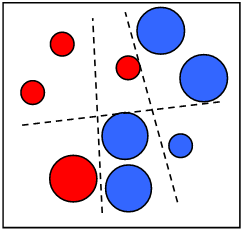
\includegraphics[scale=0.4]{adaboost}
	\caption{The three dashed lines are individually weak classifiers, since they all
	mislabel a couple of data points. However, if our model $H(x)$ uses all three classifers,
	the combined results will be quite strong.}
\end{marginfigure}

The main objective of AdaBoost is to find the model $h_{t}$ which classifies correctly 
at the highest rate. We also want to find the highest \textbf{margin} between the decision
boundary and the data points. We do this by using the negative exponent of $\alpha$.

For face detection, we sometimes use a \textbf{sliding window}, where we have a window of a 
set size and we pan it across an image to test for possible faces. However, we have comparatively
few faces in an image, and scanning that many pixels can be quite demanding.Since we have so 
many possible places for there to be a face, we can't spend that much time on any one 
individually, since that will increase our computation.

\subsection{Viola and Jones' Face Detector}
This face detector is quite influential and is the model used in real-time applications.
Its training phase is slow but the actual face detection is quite fast. We have four types
of rectangle features, which whose difference should let us know if it's likely for there 
to be a face in the image.
\begin{marginfigure}
		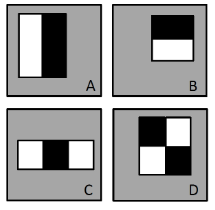
\includegraphics[scale=0.5]{rect_features}
		\caption{To quickly determine the possiblity of a face, we take the difference of the 
		white and black areas over a region of an image. These patterns roughly correspond
		to facial features.}
\end{marginfigure}

In order to quickly take the difference between the black and white areas in the figure,
we need to quickly access the individual pixel values. The \textbf{integral image} is 
a matrix where we store the sum of the  values above and to the left of pixel
$(x,y)$. This image can be quickly computed from the original image, and then to take the 
difference of an area of the image can be found with only three additions.

Using a combination of these rectangle classifiers, we can come up with a boosting model
with many parameters. We also apply an \textbf{attentional cascade} to all the positive 
subwindows. First, we apply a simple classifier, and at each stage we apply a more complex
classifier. Taking the false-positive rates of each stage in the cascade, we multiply it 
together to get an overall low false-positive rate for the entire cascade.
\end{document}
